\documentclass[a4paper,twoside]{article}

\usepackage{epsfig}
\usepackage{subfigure}
\usepackage{calc}
\usepackage{amssymb}
\usepackage{amstext}
\usepackage{amsmath}
\usepackage{amsthm}
\usepackage{multicol}
\usepackage{pslatex}
\usepackage{apalike}
\usepackage{SCITEPRESS}
\usepackage[small]{caption}
\usepackage{url}
\usepackage{graphicx}

\subfigtopskip=0pt
\subfigcapskip=0pt
\subfigbottomskip=0pt

\begin{document}

\title{SuperPhy: A Pilot Resource for Integrated Phylogenetic and Epidemiological Analysis of Pathogens}

\keywords{Bioinformatics, Computational Biology, Population Genomics, Epidemiology, Phylogeny, Bacterial Pathogenesis}

\abstract{
Advances in DNA sequencing technology have created new opportunities in fields such as clinical medicine and epidemiology, where performing real-time, genome-based surveillance and identification of phenotypic characteristics of bacterial pathogens is now possible. New analytical tools and infrastructure are needed to analyze these genomic datasets, store the data, and provide the essential biological information to end-users. We have implemented an online whole-genome analyses platform called SuperPhy that uses Panseq as an engine to compare bacterial genomes, the Fisher's exact test to identify sub-group specific loci, and FastTree to create maximum-likelihood trees. SuperPhy facilitates the upload of genomes for both private and public use. Analyses include: 1) genomic comparisons of clinical isolates, identification of virulence and antimicrobial resistance genes \textit{in silico}, 2) associations between specific genotypes and phenotypic meta-data (e.g., geospatial distribution, host, source); 3) identification of group-specific genome markers (presence/ absence of specific genomic regions, and single-nucleotide polymorphisms) in bacterial populations; 4) the ability to manipulate the display of phylogenetic trees; 5) identify statistically significant clade-specific markers. The SuperPhy pilot database currently contains genome sequences for 1063 \textit{Escherichia coli} strains.  Future work will extend SuperPhy to include multiple pathogens.}

\onecolumn \maketitle \normalsize \vfill

\section{\uppercase{Introduction}}
\label{sec:introduction}

\noindent Centralized massively parallel nucleic acid sequencing has led to an exponential increase in genome data generation that threatens to outpace advances in data storage and analysis \cite{kahn_future_2011,teeling_current_2012}. In addition, distributed bench-top sequencing platforms such as the IonTorrent and MiSeq promise to provide point of care investigation capabilities with near real-time generation of genome data \cite{loman_performance_2012}. This capability will allow us to rapidly disseminate data, especially where decisions may be time-critical; for example, in clinical medicine and epidemiological investigations. Better algorithms, more powerful analytical tools and state-of-the art infrastructure are needed to analyze these datasets, store the raw and computed data, and provide the essential biological information to a wide range of end-users in readily understandable and useful formats.

We have previously created Panseq, an online and standalone suite of software tools for the automated comparison of multiple genomes \cite{laing_pan-genome_2010,laing_identification_2011}. Panseq is based on the concept of the bacterial pan-genome. The generated outputs help elucidate our understanding of the evolution of specific bacterial groups, and the genetic basis of important phenotypic traits that differ among these groups \cite{laing_pan-genome_2010}.

In this study, we have created a complimentary computational platform, called SuperPhy (\url{http://lfz.corefacility.ca/superphy}), that provides 1) genomic comparisons of clinical isolates, identification of virulence and antimicrobial resistance genes \textit{in silico}, 2) associations between specific genotypes and phenotypic meta-data (e.g., geospatial distribution, host, source); 3) identification of group-specific genome markers (presence/ absence of specific genomic regions, and single-nucleotide polymorphisms) in bacterial populations; 4) the ability to manipulate the display of phylogenetic trees; 5) identify statistically significant clade-specific markers. In addition, SuperPhy allows private user data repositories where user-specific genome sequences and associated datasets can be uploaded and analyzed in conjunction with all public data. Figure \ref{fig:capabilities} highlights the functions of SuperPhy.

\begin{figure*}[t]
  \vspace{-0.2cm}
  \centering
   {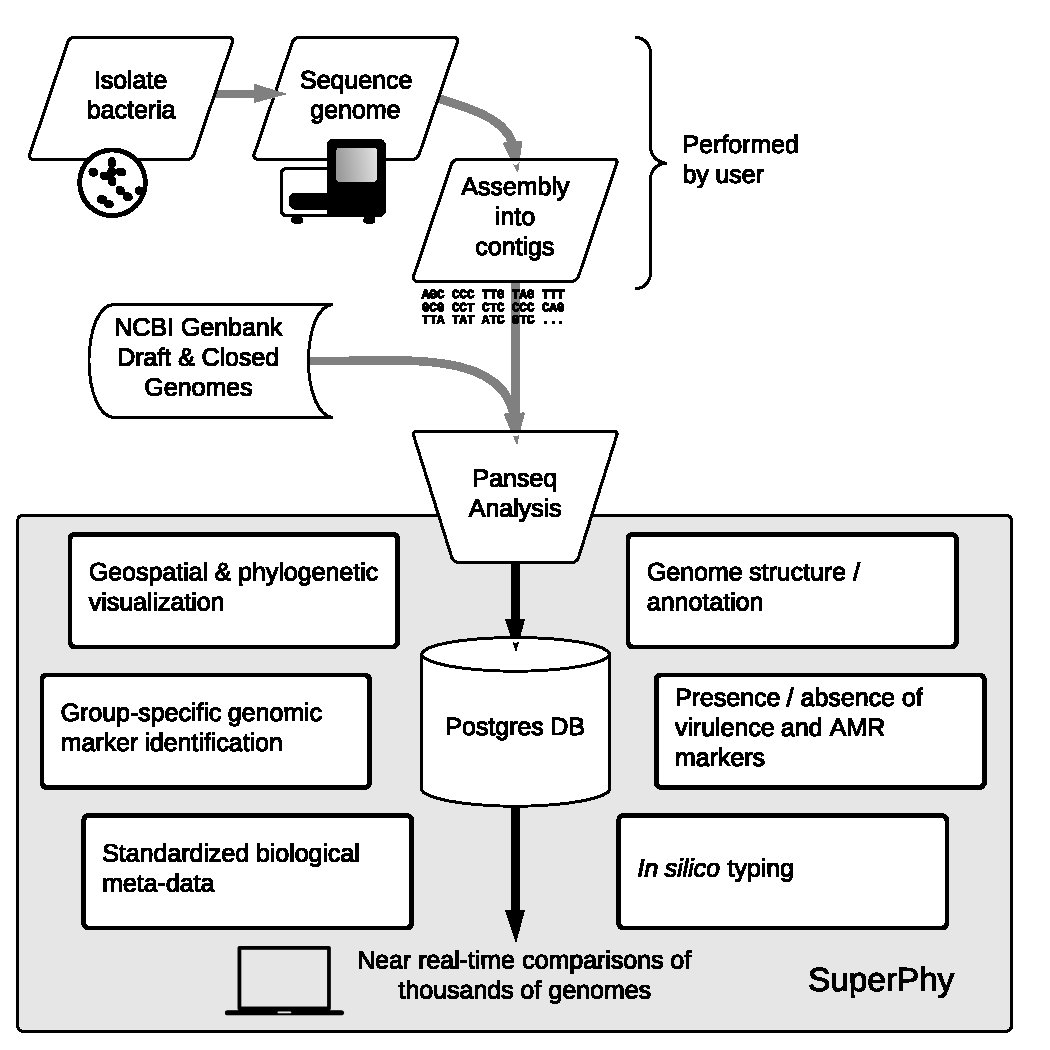
\includegraphics[width=10cm]{capabilities.pdf}}
  \caption{Overview of capabilities in the SuperPhy platform.}
  \label{fig:capabilities}
  %\vspace{-0.1cm}
\end{figure*}

The initial release of SuperPhy contains all publicly available data for \textit{Escherichia coli}, and includes expert-guided analyses of species-specific pathogroups and virulence determinants. In the future, SuperPhy will be expanded by the community to provide expert-guided analyses of additional species of bacterial pathogens for use by clinicians, epidemiologists and evolutionary biologists.

\section{\uppercase{Design}}
\label{sec:design}

\noindent SuperPhy is an interactive web platform that integrates public \textit{E. coli} genome data with analysis tools. The 1063 closed and draft \textit{E. coli} genome sequences were downloaded from GenBank and incorporated into the SuperPhy database. Users can upload their own genome sequences for analysis to be kept private, or to be integrated into the public dataset. The platform is designed to be flexible and can work with closed genomes or genomic contigs from the assembly stage. 

\subsection{Database}

The pilot stage of the SuperPhy platform focuses on analyzing genomes of \textit{E.coli}; however, SuperPhy was designed to be extensible to other species. To make the database flexible, we chose the Chado relational schema \cite{mungall2007chado}. In Chado, ontologies are used to assign types to entities, attributes and relationships \cite{mungall2007chado}. This ontology-centric design makes Chado highly adaptable. By not defining types in relational layers and instead using a mutable controlled vocabulary to assign types, the schema can be easily re-used or changed over time without having to change the relational structure \cite{mungall2007chado}.  Figure \ref{fig:ontology} shows the main entity types and corresponding relationship types used in our SuperPhy instance of the Chado schema (not shown are the attributes types). \texttt{Contig collection} is the parent term assigned to any genome project uploaded by a user or obtained from an external database and is used to store global attributes. A collection term contains one or more DNA sequences that are labelled \texttt{contig}. The \texttt{contig} types can be assembled contigs or fully closed chromosomes or plasmids. In SuperPhy, further experimental features are calculated for each genome: pan-genome loci, antimicrobial resistance genes, virulence factor alleles, and single nucleotide polymorphisms (SNPs) in the core genome.

A predefined set of required and optional genome meta-data fields and permissible values have been selected from the minimum information about a genome sequence (MIGS) specification \cite{field2008}. The meta-data types capture key bacterial isolate attributes.

\begin{figure*}[t]
  \vspace{-0.2cm}
  \centering
   {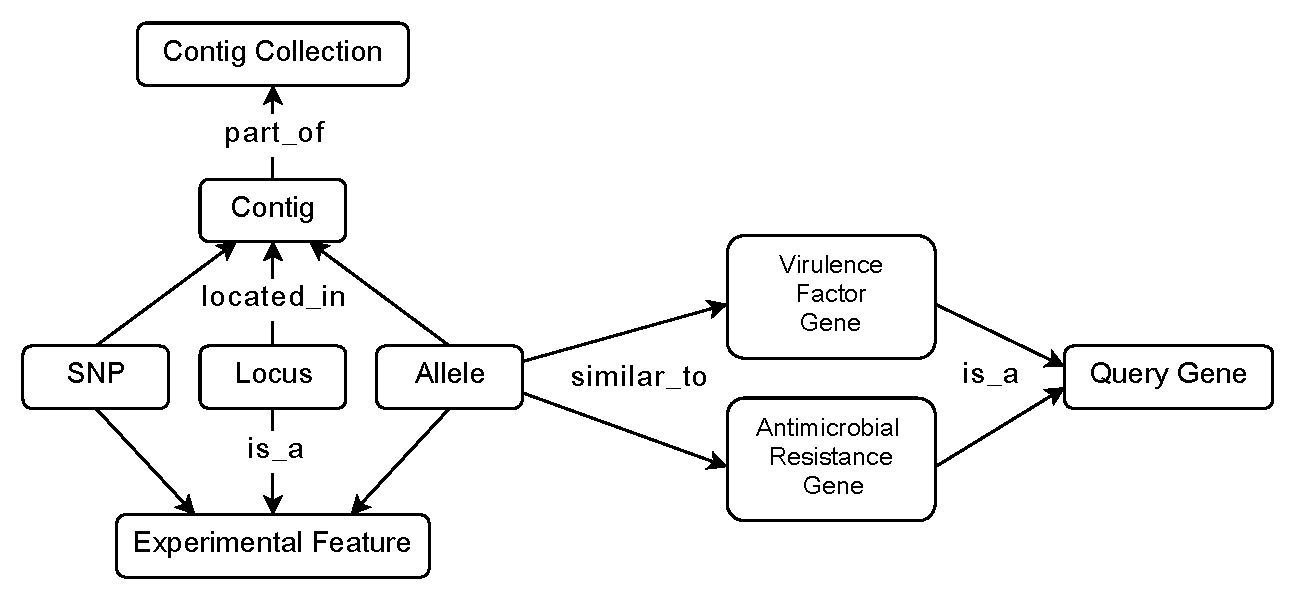
\epsfig{file = ontology.eps, width = 12cm}}
  \caption{A ontology graph representing the main entity types used in the SuperPhy schema.}
  \label{fig:ontology}
  %\vspace{-0.1cm}
\end{figure*}

\subsection{Analyses}
\label{sec:pipeline}

Panseq is used as the computational engine for the SuperPhy platform \cite{laing_pan-genome_2010}. Genome sequences uploaded by users or obtained from NCBI GenBank Genome and Whole Genome Sequence repositories \cite{benson2013genbank} are input into Panseq to identify segments that belong to the conserved core genome and to the more variable accessory genome. Panseq works by iteratively aligning genomes using the MUMmer 3 program to produce a non-redundant pan-genome sequence \cite{laing_pan-genome_2010,kurtz2004versatile}. The pan-genome is then compared back to the input genomes to generate a listing of the presence or absence of each genomic locus in the pan-genome across the input genomes. Panseq also catalogues the SNP variations in the conserved regions \cite{laing_pan-genome_2010}.  The loci and SNPs identified by Panseq are loaded into the SuperPhy database. Annotations for the pan-genome regions are determined using a BLASTx analysis against the GenBank NR protein database.

A second analysis identifies virulence and antimicrobial drug resistance determinants in the genomes. Starting with a predefined set of query virulence factor (VF) and antimicrobial resistance (AMR) genes, the Panseq tool searches for alleles of these genes in the input genomes. Panseq uses BLASTn to conduct the search. The non-redundant query set of AMR genes was created by downloading the entire Comprehensive Antibiotic Resistance Database (CARD) \cite{mcarthur2012card} and subsequently clustering the CARD sequences based on similarity using BLASTclust \cite{altschul_gapped_1997}. Representatives from each cluster were selected first by the phylogenetic distance of the species to \textit{E. coli} and secondly, by length where longer sequences were selected over shorter ones. All query AMR genes are organized according to their Antibiotic Resistance Ontology annotation to aid in identifying the presence of different antimicrobial resistance mechanisms \cite{antezana_biological_2009}. The VF gene set was produced by obtaining all gene alleles of known virulence factors in \textit{E. coli} from the Virulence Factor Database \cite{chen2012vfdb,chen2005vfdb}.  The longest allele was selected for each VF gene, except in cases where sequence similarity was less than 90\%, in which case, multiple alleles were included in the VF query set for a particular gene.

Phylogenetic trees in SuperPhy are used in the results displays and also in the query forms. A maximum-likelihood phylogenetic tree is constructed for all \textit{E. coli} genomes in the database using FastTree v2.1 \cite{price_fasttree_2010}. The tree is built from a multiple sequence alignment of the conserved core genome regions among all genomes, but is dynamically pruned based on user-selection to show specific genomes. Trees are also computed for individual pan-genome regions and for identified AMR and VF genes.

Shiga-toxin (Stx) subtype assignment of the \textit{E. coli} strains is calculated from the phylogenetic distribution of the query alleles in relation to Stx genes with confirmed subtype. A phylogenetic tree of all identified \textit{stx1} and \textit{stx2} was created, and clades specific to a Shiga-toxin subtype were identified based on the scheme presented by \cite{scheutz_multicenter_2012}. Membership in these pre-defined clades marks the subtype of a genome; those strains that fall outside of known sub-type clades are marked as unknown. Multiple sequence alignments of the Stx genes are stored in the database for user reference.

\subsection{Implementation Details}

The web application was built with the Perl CGI::Application framework (\url{http://cgi-app.org/}). The Chado relational database schema was implemented in Postgres 9.2. The Phylogenetic tree graphical display is constructed with the D\sup{3} JavaScript library \cite{bostock2011d3} and the map tool with the Google Maps JavaScript API v3 (\url{https://developers.google.com/maps/documentation/javascript/}).

\section{\uppercase{Functionality}}
\label{sec:functionality}

\subsection{Uploading a Genome}

Users can upload their \textit{E. coli} genomes to SuperPhy for analysis and comparison to the other \textit{E. coli} genomes in the database.  Access to uploaded genomes and associated analyses is regulated by the user. Users can select to keep their genome data private indefinitely, immediately make it publicly accessible, or choose to release it after a specified date, where it will automatically be added to the public data.  Under the private setting, users can also grant specific users access to their genomes. After upload, genomes are submitted to the SuperPhy analysis pipeline. Return times for the results depend on server load, but under typical conditions, analysis results are available within an hour.

\subsection{Retrieving Genome Meta-data}

Existing \textit{E. coli} genomes from the NCBI GenBank and Whole Genome Sequence repositories \cite{benson2013genbank} have been loaded into the SuperPhy database. Meta-data in these sources were mapped to the standardized MIGS set of meta-data types and values \cite{field2008}. To facilitate navigation, users can choose to display one or more meta-data types in the forms (accession, serotype, strain, host species, isolation source, isolate date can be displayed alongside genome name). Through the advanced search facility, genome information can be queried by selecting from a interactive phylogenetic tree, from a world map, by date range or by boolean search of user-defined search fields and keywords.  The sophisticated query interface is designed to help address a broad range of hypotheses based on meta-data or phylogenetic information (Figure \ref{fig:search}).

\begin{figure*}[t]
  \vspace{-0.2cm}
  \centering
   {\includegraphics[width=14cm]{superphy_forms_copy.pdf}}
  \caption{Advanced search function in SuperPhy. Genome information can be queried by (A) interactive phylogenetic tree (B) world map or (C) boolean search of user-specified fields and keywords.}
  \label{fig:search}
  %\vspace{-0.1cm}
\end{figure*}


\subsection{Groupwise Comparisons of the Distribution of SNPs and the Presence / Absence of Variable Genomic Loci}

The \textit{E. coli} pan-genome is highly variable, with approximately 80\% of an individual genome comprised of variable, accessory genes and only 20\% from the core-genome \cite{lukjancenko_comparison_2010}. To help correlate phenotype and genotype, SuperPhy provides the ability to compare between groups the presence or absence of pan-genome loci, as well as the distribution of SNPs within shared genome regions. A single consolidated pan-genome is computed from the individual genomes in the SuperPhy database. To identify group-specific or group-dominant genome regions or SNPs, the groupwise comparison function of SuperPhy allows users to select genomes in two comparison groups and returns the set of nucleotide variations or genome regions that are statistically enriched in one group compared to the other. The statistical enrichment is determined by the Fisher's Exact test as implemented in the R statistical language \cite{R_manual}.

\subsection{Identifying Virulence and Antimicrobial Drug Resistance Determinants}

SuperPhy provides the ability to identify and evaluate risk factors. Users can examine the distribution of the presence or absence of virulence and AMR markers in the genomes.  Pre-defined sets of characterized virulence factors and antimicrobial resistance genes were collected and examined for their presence among all individual genomes \cite{mcarthur2012card,chen2012vfdb,chen2005vfdb}. Users can specify multiple query markers in multiple target genomes. The sequences of identified VF and AMR gene alleles in the individual genomes are stored in the database, as are the multiple sequence alignments of the alleles. This allows the sequence-based comparison among user selected strains to be displayed in real-time.

\subsection{Visualizing Phylogenetic and Geospatial Data}

Phylogenetic tree views are provided for Genomes, AMR and VF genes and individual pan-genome regions (Figure \ref{fig:search}A). The tree interface is designed to be highly interactive; users can pan, zoom and expand, collapse or select tree nodes. The tree view is coupled with an interactive world map view of the location of strains (Figure \ref{fig:search}B). Locations can be regions such as countries, territories or states, or can be points defined by latitude and longitude coordinates. Queried genomes are simultaneously displayed in the tree and map views allowing users to explore and compare the phylogenetic and geospatial positions of strains. Meta-data such as host, source, associated disease or isolation date can be overlayed in the phylogenetic tree.

\subsection{Shiga-Toxin Subtyping}

Shiga-Toxin (Stx) producing \textit{E.coli} can be characterized by their Stx1 and Stx2 gene variants \cite{scheutz_multicenter_2012}. Stx variants are often associated with distinct biological phenotypes. Stx subtypes are assigned to the Shiga-toxin \textit{E.coli} in the database based on the cluster membership of the Stx alleles in predefined phylogenetic clades in the Stx gene tree. Stx subtype is presented on the Strain Information summary page, where a phylogenetic tree of the Stx genes can also be viewed.

\section{\uppercase{Examples of Use Cases}}
\label{sec:cases}
\subsection{Time Critical Genomic Analyses}
Example: A clinician has just received a bacterial isolate from a patient with gastrointestinal illness and would like to know the risk to the patient (how severe and what sort of illness is associated with the strain based on meta-data from closely related strains in the database), the risk to the community (have these bacteria been isolated from other patients; is this an outbreak?) and possible treatment or prevention options. In order for the information to be to useful, the bacterial isolate must be characterized as soon as possible. The genome sequence is determined in the hospital using a distributed sequencing platform such as the MiSeq or IonTorrent and subsequently uploaded to SuperPhy. The resulting information presented contains a summary of the strain for known virulence and AMR determinants, any novel genome regions with respect to the genomes already present in the database, the phylogenetic position of the new isolate and closely related strains, and their geographical distribution. This clinician also has the opportunity to add the new strain to the shared public database, where it will instantly be available to the community of SuperPhy users.

In the current genomics landscape, it is impossible to perform the above analyses in the time required to make effective decisions. The same analyses would require days of wet-lab work, and to perform these tasks \textit{in silico}, one would need knowledge of a number of bioinformatics programs, a local collection of strains to run the comparison against, a collection of virulence and antimicrobial factors, and a means of identifying unique genome elements.

The entire process would be lengthy and the knowledge gained would not be immediately available to others. With our novel integration of the data and computational approaches, the analyses can be performed relatively quickly, a summary generated, and both the genome and
information about that genome stored and available for other users, saving duplication of analyses and increasing the value of the computational platform. The rate-limiting step for the platform is now the deposition of genome sequence data.

\subsection{Identification of Genomic Novelty Informing Phenotype}
Examples: 1) An epidemiologist has identified a pathogen responsible for high levels of severe illness and wishes to identify genome regions that are present in the pathogen but absent among closely related strains not implicated in human disease; 2) An agricultural researcher wishes to identify genome elements statistically associated with \textit{E. coli} strains that are shed from cattle more frequently and in higher amounts than other \textit{E. coli} found in the bovine gastrointestinal tract; 3) A researcher wishes to identify novel genes in a group of \textit{E. coli} that persist in soil longer than other known groups of \textit{E. coli}; 4) A food microbiologist wishes to identify genome regions that allow persistent \textit{E. coli} to remain in a food-production environment, where most other \textit{E. coli} are not capable of persisting.

As the SuperPhy computational tools are tightly coupled with the underlying data, all meta-data (source, host, severity of illness, etc.) are immediately available for determining phenotypic groups that can be compared at the genome level. Additionally, the spatial distribution of genome sequences is displayed in map form, allowing the user to `zoom-in' and graphically select a region of interest. The presence / absence of all genome regions and single-nucleotide polymorphisms among shared genome regions is also pre-computed, enabling the identification of genome regions that are statistically different between groups, be they based on severity of illness, host, or geographical location.

The results are then made available for download and the analysis saved in the platform for others to use with permission of the original user.

\subsection{Discovery Research}
Example: A genomics researcher has obtained the assembled contigs from an Illumina sequencing run, generating a large number of novel genome sequences in a novel \textit{E. coli} strain responsible for severe cases of human disease, as was seen in the 2011 \textit{E. coli} O104:H4 outbreak \cite{mellmann_prospective_2011}. He wishes to quickly identify the phylogenetic relationships among this new strain and all previously sequenced \textit{E. coli} genomes, as well as to identify virulence and AMR genes, and novel genomic regions present in the strains with respect to closely related genome sequences. The researcher simply uploads his sequences to SuperPhy, after which the new strains are placed on the phylogenetic tree of all strains, and the presence of any known virulence / AMR genes is determined. Lastly, the new strains are compared to the pre-computed genomes database, where any novel genomic regions are identified for the researcher.

\section{\uppercase{Discussion}}
\label{sec:discussion}

To meet the opportunities presented by current genome sequencing technologies, tools are needed that can analyze genomic data in a rapid and accessible way. Efforts have been made to automate complex bioinformatics workflows, such as Taverna \cite{lanzen_taverna_2008} and Galaxy \cite{goecks_galaxy:_2010}, and while they are effective at simplifying the process, data are not integrated with these tools requiring users to transfer genome sequences from public or private databases and perform their own separate analyses. Likewise, online repositories of genome sequence data such as the National Center for Biotechnology Information (\url{http://www.ncbi.nlm.nih.gov/}) and the Genomes Online Database (\url{http://www.genomesonline.org/}) provide a wealth of data, but are decoupled from an efficient analytical platform. 

Only recently have platforms emerged that attempt to provide both large-scale data storage and analyses. Relevant to microbiology, the tools MicroScope and PATRIC provide broad pre-computed analyses for public genomes \cite{vallenet_microscope--integrated_2012,wattam2013}.  MicroScope, limited to publicly available closed and annotated genomes, contains information for $>$1100 genomes, while PATRIC, which has a gene annotation workflow and includes incomplete genomes, contains $>$10 000 genome sequences. Analysis results compare the phylogeny, biological pathways and gene functions of bacterial species. Several of the analyses in MicroScope focus on comparing the genome structure. Both tools allow users to add genome-associated data such as transcriptomics results to aid in the understanding of gene function \cite{vallenet_microscope--integrated_2012,wattam2013}. 

IMG is a combined genome annotation and analysis platform \cite{marko2013}. While more limited in scope in comparison to PATRIC or MicroScope, IMG allows the submission of genomic data by users. Other platforms are organism specific, such as Sybil; a platform for the comparative analyses of \textit{Streptococcus pneumoniae} based on BLASTp searches \cite{riley_using_2012}. Outside of these broad analyses suites, other large-scale genome tools tend to focus on a specific analysis. For example, several tools provide a global phylogenetic tree for public bacterial genomes \cite{letunic2011,fang2013,federhen2012}.

The integration of phylogenetic and epidemiological analyses with genomic data uniquely positions SuperPhy to aid both clinical and basic microbiological research. Users can upload their incomplete or closed genomic sequence data and in near real-time compare their strain to other public or user-submitted strains in the database. Analyses provided clear, targeted answers to questions that are of interest to microbiologists and clinicians.  The group-based comparison allows users to investigate genotype-phenotype correlations, by statistically evaluating associated genomic markers or regions in user-supplied strain groups. While other platforms can identify SNPs or novel regions, SuperPhy evaluates the significance of genomic novelty in the context of the comparison groups. SuperPhy contains lists of known disease risk factors and highlights the presence or absence of the factors. Relevant pathogen-specific data is also incorporated into SuperPhy; shiga-toxin \textit{E.coli} variants are characterized using an \textit{in silico} typing method. Finally, result are displayed in integrated, information-rich, but understandable views. Retrieving the information for a strain, for example, will return a geographical map, a phylogenetic tree and all associated meta-data (e.g source, host, associated diseases, Stx subtype, Pubmed ID, etc.). In the tree and map views, meta-data can be overlayed to examine the distribution of a particular feature.  Retrieving similar information on other platforms would require significant manipulation or manual collation of data across analysis tools. In coupling data with targeted analysis tools and result views, SuperPhy can quickly obtain answers to multiple research hypotheses, by users with little bioinformatics expertise.

\subsection{Collaboration and Community Benefit}
\label{sec:collaboration}
There are currently similar projects under way world-wide with similar goals: to provide a platform for comparative genomic epidemiology \cite{kupferschmidt_outbreak_2011}. The transfer of strains across international borders can be time consuming or impossible, whereas the exchange of genome sequence information can happen as soon as it becomes available. These international efforts with common goals should at the least provide data in a format that allows for it to be easily shared and understood among the various platforms. The value to the community of users of this shared computational resource increases as the number of users contributing data to it increases, which in turn makes the platform more attractive to use and contribute to by others. Users are encouraged to add not only data, but suggest improvements and additions to the SuperPhy platform, so that it can be iteratively developed to meet the needs of the user community.

\section{\uppercase{Availability}}
\label{sec:availability}

The website is available at http://lfz.corefacility.ca/superphy/. The software code and database will be made available upon request.

\section{\uppercase{Conclusions}}
\label{sec:conclusion}

\noindent SuperPhy is a broadly accessible, integrated platform for the phylogenetic and epidemiological analyses of bacterial genome data. It provides near real-time analyses of thousands of genome sequences using novel computational approaches with results that are understandable and useful to a wide community, including those in the fields of clinical medicine, epidemiology, ecology and evolution. The web-interface to this computational platform obviates the need for command-line skills, or a particular computer environment. As additional members of the research community use the platform, the number of genome sequences stored and analyzed will increase, adding further value to the platform, and in turn attracting more users. Genomic platforms such as SuperPhy will become increasingly important in transforming raw genome data into a format suitable for the development of a world-wide real-time surveillance and analyses network for bacterial genomes.

\vfill
\bibliographystyle{apalike}
{\small
\bibliography{bioinformatics2014}}

\vfill
\end{document}
